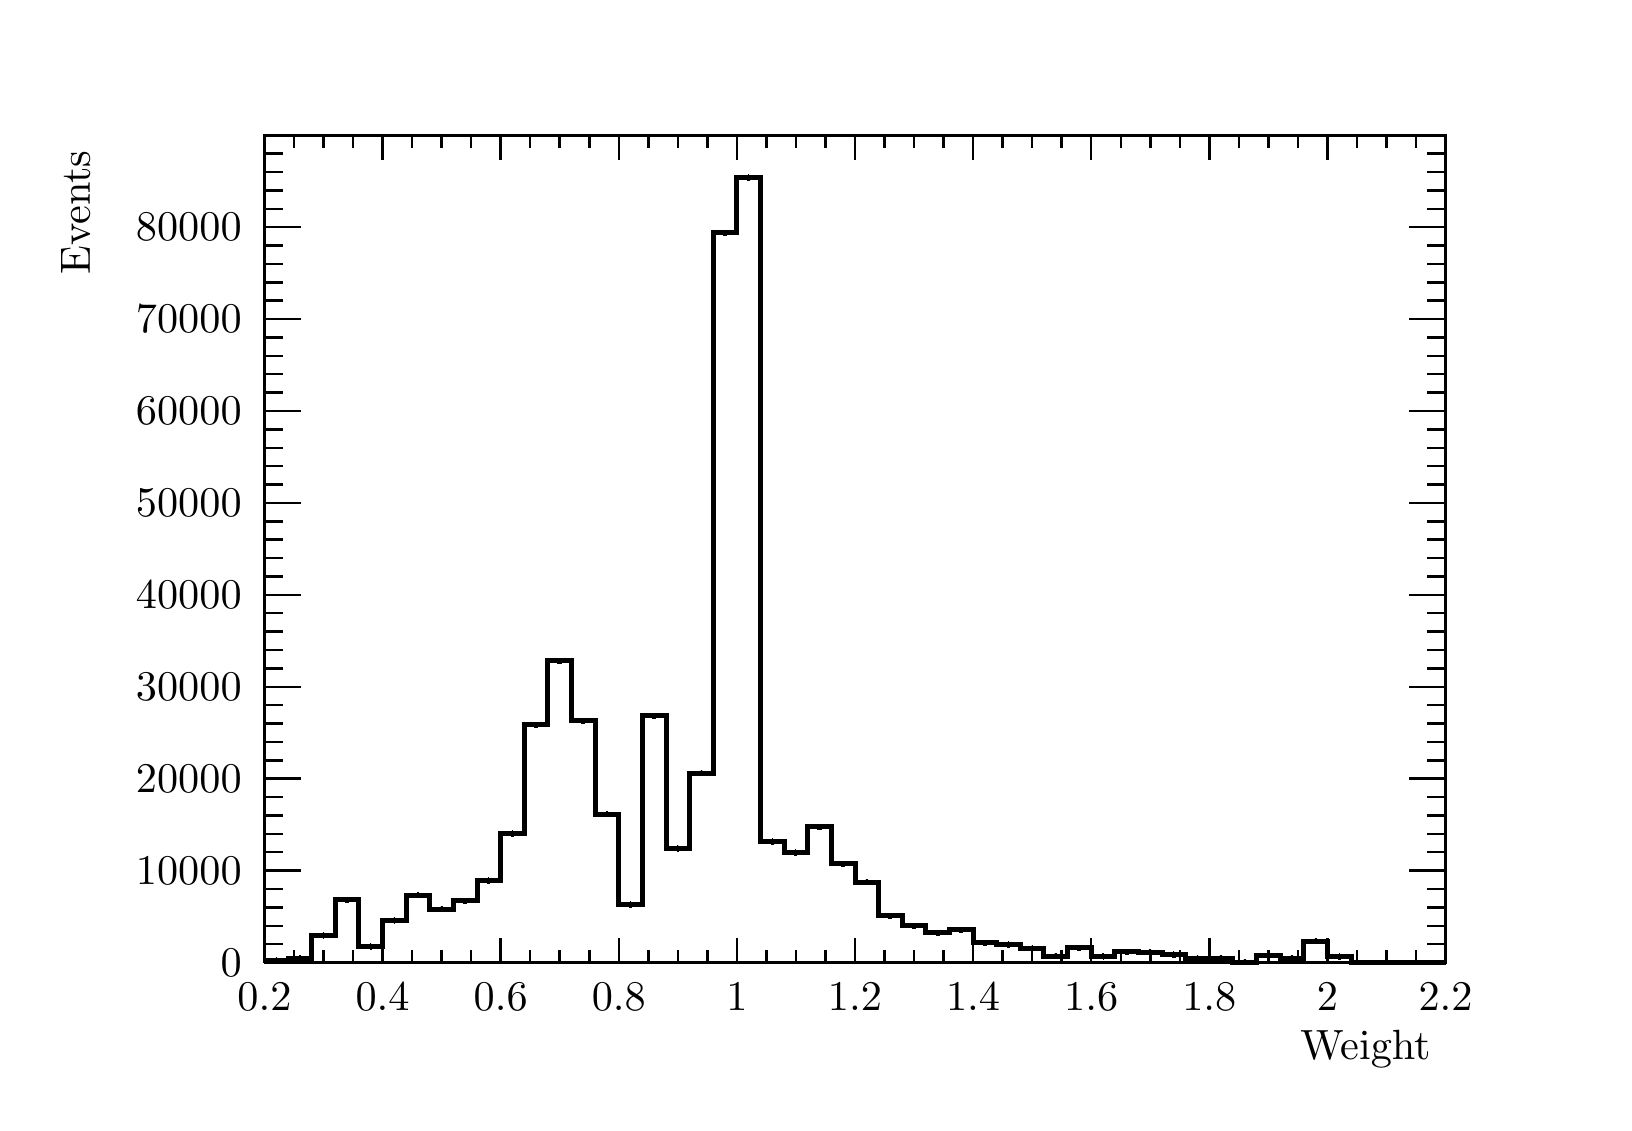
\begin{tikzpicture}
\pgfdeclareplotmark{cross} {
\pgfpathmoveto{\pgfpoint{-0.3\pgfplotmarksize}{\pgfplotmarksize}}
\pgfpathlineto{\pgfpoint{+0.3\pgfplotmarksize}{\pgfplotmarksize}}
\pgfpathlineto{\pgfpoint{+0.3\pgfplotmarksize}{0.3\pgfplotmarksize}}
\pgfpathlineto{\pgfpoint{+1\pgfplotmarksize}{0.3\pgfplotmarksize}}
\pgfpathlineto{\pgfpoint{+1\pgfplotmarksize}{-0.3\pgfplotmarksize}}
\pgfpathlineto{\pgfpoint{+0.3\pgfplotmarksize}{-0.3\pgfplotmarksize}}
\pgfpathlineto{\pgfpoint{+0.3\pgfplotmarksize}{-1.\pgfplotmarksize}}
\pgfpathlineto{\pgfpoint{-0.3\pgfplotmarksize}{-1.\pgfplotmarksize}}
\pgfpathlineto{\pgfpoint{-0.3\pgfplotmarksize}{-0.3\pgfplotmarksize}}
\pgfpathlineto{\pgfpoint{-1.\pgfplotmarksize}{-0.3\pgfplotmarksize}}
\pgfpathlineto{\pgfpoint{-1.\pgfplotmarksize}{0.3\pgfplotmarksize}}
\pgfpathlineto{\pgfpoint{-0.3\pgfplotmarksize}{0.3\pgfplotmarksize}}
\pgfpathclose
\pgfusepathqstroke
}
\pgfdeclareplotmark{cross*} {
\pgfpathmoveto{\pgfpoint{-0.3\pgfplotmarksize}{\pgfplotmarksize}}
\pgfpathlineto{\pgfpoint{+0.3\pgfplotmarksize}{\pgfplotmarksize}}
\pgfpathlineto{\pgfpoint{+0.3\pgfplotmarksize}{0.3\pgfplotmarksize}}
\pgfpathlineto{\pgfpoint{+1\pgfplotmarksize}{0.3\pgfplotmarksize}}
\pgfpathlineto{\pgfpoint{+1\pgfplotmarksize}{-0.3\pgfplotmarksize}}
\pgfpathlineto{\pgfpoint{+0.3\pgfplotmarksize}{-0.3\pgfplotmarksize}}
\pgfpathlineto{\pgfpoint{+0.3\pgfplotmarksize}{-1.\pgfplotmarksize}}
\pgfpathlineto{\pgfpoint{-0.3\pgfplotmarksize}{-1.\pgfplotmarksize}}
\pgfpathlineto{\pgfpoint{-0.3\pgfplotmarksize}{-0.3\pgfplotmarksize}}
\pgfpathlineto{\pgfpoint{-1.\pgfplotmarksize}{-0.3\pgfplotmarksize}}
\pgfpathlineto{\pgfpoint{-1.\pgfplotmarksize}{0.3\pgfplotmarksize}}
\pgfpathlineto{\pgfpoint{-0.3\pgfplotmarksize}{0.3\pgfplotmarksize}}
\pgfpathclose
\pgfusepathqfillstroke
}
\pgfdeclareplotmark{newstar} {
\pgfpathmoveto{\pgfqpoint{0pt}{\pgfplotmarksize}}
\pgfpathlineto{\pgfqpointpolar{44}{0.5\pgfplotmarksize}}
\pgfpathlineto{\pgfqpointpolar{18}{\pgfplotmarksize}}
\pgfpathlineto{\pgfqpointpolar{-20}{0.5\pgfplotmarksize}}
\pgfpathlineto{\pgfqpointpolar{-54}{\pgfplotmarksize}}
\pgfpathlineto{\pgfqpointpolar{-90}{0.5\pgfplotmarksize}}
\pgfpathlineto{\pgfqpointpolar{234}{\pgfplotmarksize}}
\pgfpathlineto{\pgfqpointpolar{198}{0.5\pgfplotmarksize}}
\pgfpathlineto{\pgfqpointpolar{162}{\pgfplotmarksize}}
\pgfpathlineto{\pgfqpointpolar{134}{0.5\pgfplotmarksize}}
\pgfpathclose
\pgfusepathqstroke
}
\pgfdeclareplotmark{newstar*} {
\pgfpathmoveto{\pgfqpoint{0pt}{\pgfplotmarksize}}
\pgfpathlineto{\pgfqpointpolar{44}{0.5\pgfplotmarksize}}
\pgfpathlineto{\pgfqpointpolar{18}{\pgfplotmarksize}}
\pgfpathlineto{\pgfqpointpolar{-20}{0.5\pgfplotmarksize}}
\pgfpathlineto{\pgfqpointpolar{-54}{\pgfplotmarksize}}
\pgfpathlineto{\pgfqpointpolar{-90}{0.5\pgfplotmarksize}}
\pgfpathlineto{\pgfqpointpolar{234}{\pgfplotmarksize}}
\pgfpathlineto{\pgfqpointpolar{198}{0.5\pgfplotmarksize}}
\pgfpathlineto{\pgfqpointpolar{162}{\pgfplotmarksize}}
\pgfpathlineto{\pgfqpointpolar{134}{0.5\pgfplotmarksize}}
\pgfpathclose
\pgfusepathqfillstroke
}
\definecolor{c}{rgb}{1,1,1};
\draw [color=c, fill=c] (0,0) rectangle (20,13.639);
\draw [color=c, fill=c] (3,1.77307) rectangle (18,12.2751);
\definecolor{c}{rgb}{0,0,0};
\draw [c,line width=0.9] (3,1.77307) -- (3,12.2751) -- (18,12.2751) -- (18,1.77307) -- (3,1.77307);
\definecolor{c}{rgb}{1,1,1};
\draw [color=c, fill=c] (3,1.77307) rectangle (18,12.2751);
\definecolor{c}{rgb}{0,0,0};
\draw [c,line width=0.9] (3,1.77307) -- (3,12.2751) -- (18,12.2751) -- (18,1.77307) -- (3,1.77307);
\draw [c,line width=1.8] (3.15,1.79578) -- (3.15,1.79746);
\draw [c,line width=1.8] (3.15,1.79746) -- (3.15,1.79915);
\foreach \P in {(3.15,1.79746)}{\draw[mark options={color=c,fill=c},mark size=2.402402pt, line width=0.000000pt, mark=*,mark size=1pt] plot coordinates {\P};}
\draw [c,line width=1.8] (3.45,1.82552) -- (3.45,1.82805);
\draw [c,line width=1.8] (3.45,1.82805) -- (3.45,1.83058);
\foreach \P in {(3.45,1.82805)}{\draw[mark options={color=c,fill=c},mark size=2.402402pt, line width=0.000000pt, mark=*,mark size=1pt] plot coordinates {\P};}
\draw [c,line width=1.8] (3.75,2.1118) -- (3.75,2.11815);
\draw [c,line width=1.8] (3.75,2.11815) -- (3.75,2.12449);
\foreach \P in {(3.75,2.11815)}{\draw[mark options={color=c,fill=c},mark size=2.402402pt, line width=0.000000pt, mark=*,mark size=1pt] plot coordinates {\P};}
\draw [c,line width=1.8] (4.05,2.55796) -- (4.05,2.56759);
\draw [c,line width=1.8] (4.05,2.56759) -- (4.05,2.57723);
\foreach \P in {(4.05,2.56759)}{\draw[mark options={color=c,fill=c},mark size=2.402402pt, line width=0.000000pt, mark=*,mark size=1pt] plot coordinates {\P};}
\draw [c,line width=1.8] (4.35,1.97294) -- (4.35,1.97783);
\draw [c,line width=1.8] (4.35,1.97783) -- (4.35,1.98272);
\foreach \P in {(4.35,1.97783)}{\draw[mark options={color=c,fill=c},mark size=2.402402pt, line width=0.000000pt, mark=*,mark size=1pt] plot coordinates {\P};}
\draw [c,line width=1.8] (4.65,2.30145) -- (4.65,2.30937);
\draw [c,line width=1.8] (4.65,2.30937) -- (4.65,2.31728);
\foreach \P in {(4.65,2.30937)}{\draw[mark options={color=c,fill=c},mark size=2.402402pt, line width=0.000000pt, mark=*,mark size=1pt] plot coordinates {\P};}
\draw [c,line width=1.8] (4.95,2.61808) -- (4.95,2.62807);
\draw [c,line width=1.8] (4.95,2.62807) -- (4.95,2.63806);
\foreach \P in {(4.95,2.62807)}{\draw[mark options={color=c,fill=c},mark size=2.402402pt, line width=0.000000pt, mark=*,mark size=1pt] plot coordinates {\P};}
\draw [c,line width=1.8] (5.25,2.44277) -- (5.25,2.45167);
\draw [c,line width=1.8] (5.25,2.45167) -- (5.25,2.46057);
\foreach \P in {(5.25,2.45167)}{\draw[mark options={color=c,fill=c},mark size=2.402402pt, line width=0.000000pt, mark=*,mark size=1pt] plot coordinates {\P};}
\draw [c,line width=1.8] (5.55,2.5459) -- (5.55,2.55545);
\draw [c,line width=1.8] (5.55,2.55545) -- (5.55,2.56501);
\foreach \P in {(5.55,2.55545)}{\draw[mark options={color=c,fill=c},mark size=2.402402pt, line width=0.000000pt, mark=*,mark size=1pt] plot coordinates {\P};}
\draw [c,line width=1.8] (5.85,2.80254) -- (5.85,2.81356);
\draw [c,line width=1.8] (5.85,2.81356) -- (5.85,2.82459);
\foreach \P in {(5.85,2.81356)}{\draw[mark options={color=c,fill=c},mark size=2.402402pt, line width=0.000000pt, mark=*,mark size=1pt] plot coordinates {\P};}
\draw [c,line width=1.8] (6.15,3.39686) -- (6.15,3.41069);
\draw [c,line width=1.8] (6.15,3.41069) -- (6.15,3.42451);
\foreach \P in {(6.15,3.41069)}{\draw[mark options={color=c,fill=c},mark size=2.402402pt, line width=0.000000pt, mark=*,mark size=1pt] plot coordinates {\P};}
\draw [c,line width=1.8] (6.45,4.77248) -- (6.45,4.79125);
\draw [c,line width=1.8] (6.45,4.79125) -- (6.45,4.81002);
\foreach \P in {(6.45,4.79125)}{\draw[mark options={color=c,fill=c},mark size=2.402402pt, line width=0.000000pt, mark=*,mark size=1pt] plot coordinates {\P};}
\draw [c,line width=1.8] (6.75,5.58203) -- (6.75,5.60317);
\draw [c,line width=1.8] (6.75,5.60317) -- (6.75,5.62432);
\foreach \P in {(6.75,5.60317)}{\draw[mark options={color=c,fill=c},mark size=2.402402pt, line width=0.000000pt, mark=*,mark size=1pt] plot coordinates {\P};}
\draw [c,line width=1.8] (7.05,4.82415) -- (7.05,4.84308);
\draw [c,line width=1.8] (7.05,4.84308) -- (7.05,4.86201);
\foreach \P in {(7.05,4.84308)}{\draw[mark options={color=c,fill=c},mark size=2.402402pt, line width=0.000000pt, mark=*,mark size=1pt] plot coordinates {\P};}
\draw [c,line width=1.8] (7.35,3.64264) -- (7.35,3.65747);
\draw [c,line width=1.8] (7.35,3.65747) -- (7.35,3.67231);
\foreach \P in {(7.35,3.65747)}{\draw[mark options={color=c,fill=c},mark size=2.402402pt, line width=0.000000pt, mark=*,mark size=1pt] plot coordinates {\P};}
\draw [c,line width=1.8] (7.65,2.49937) -- (7.65,2.50864);
\draw [c,line width=1.8] (7.65,2.50864) -- (7.65,2.51791);
\foreach \P in {(7.65,2.50864)}{\draw[mark options={color=c,fill=c},mark size=2.402402pt, line width=0.000000pt, mark=*,mark size=1pt] plot coordinates {\P};}
\draw [c,line width=1.8] (7.95,4.8863) -- (7.95,4.90542);
\draw [c,line width=1.8] (7.95,4.90542) -- (7.95,4.92454);
\foreach \P in {(7.95,4.90542)}{\draw[mark options={color=c,fill=c},mark size=2.402402pt, line width=0.000000pt, mark=*,mark size=1pt] plot coordinates {\P};}
\draw [c,line width=1.8] (8.25,3.21042) -- (8.25,3.22344);
\draw [c,line width=1.8] (8.25,3.22344) -- (8.25,3.23645);
\foreach \P in {(8.25,3.22344)}{\draw[mark options={color=c,fill=c},mark size=2.402402pt, line width=0.000000pt, mark=*,mark size=1pt] plot coordinates {\P};}
\draw [c,line width=1.8] (8.55,4.16126) -- (8.55,4.17802);
\draw [c,line width=1.8] (8.55,4.17802) -- (8.55,4.19477);
\foreach \P in {(8.55,4.17802)}{\draw[mark options={color=c,fill=c},mark size=2.402402pt, line width=0.000000pt, mark=*,mark size=1pt] plot coordinates {\P};}
\draw [c,line width=1.8] (8.85,11.0081) -- (8.85,11.041);
\draw [c,line width=1.8] (8.85,11.041) -- (8.85,11.0739);
\foreach \P in {(8.85,11.041)}{\draw[mark options={color=c,fill=c},mark size=2.402402pt, line width=0.000000pt, mark=*,mark size=1pt] plot coordinates {\P};}
\draw [c,line width=1.8] (9.15,11.7068) -- (9.15,11.7409);
\draw [c,line width=1.8] (9.15,11.7409) -- (9.15,11.775);
\foreach \P in {(9.15,11.7409)}{\draw[mark options={color=c,fill=c},mark size=2.402402pt, line width=0.000000pt, mark=*,mark size=1pt] plot coordinates {\P};}
\draw [c,line width=1.8] (9.45,3.29515) -- (9.45,3.30854);
\draw [c,line width=1.8] (9.45,3.30854) -- (9.45,3.32193);
\foreach \P in {(9.45,3.30854)}{\draw[mark options={color=c,fill=c},mark size=2.402402pt, line width=0.000000pt, mark=*,mark size=1pt] plot coordinates {\P};}
\draw [c,line width=1.8] (9.75,3.15604) -- (9.75,3.1688);
\draw [c,line width=1.8] (9.75,3.1688) -- (9.75,3.18157);
\foreach \P in {(9.75,3.1688)}{\draw[mark options={color=c,fill=c},mark size=2.402402pt, line width=0.000000pt, mark=*,mark size=1pt] plot coordinates {\P};}
\draw [c,line width=1.8] (10.05,3.48149) -- (10.05,3.49567);
\draw [c,line width=1.8] (10.05,3.49567) -- (10.05,3.50985);
\foreach \P in {(10.05,3.49567)}{\draw[mark options={color=c,fill=c},mark size=2.402402pt, line width=0.000000pt, mark=*,mark size=1pt] plot coordinates {\P};}
\draw [c,line width=1.8] (10.35,3.01347) -- (10.35,3.02556);
\draw [c,line width=1.8] (10.35,3.02556) -- (10.35,3.03766);
\foreach \P in {(10.35,3.02556)}{\draw[mark options={color=c,fill=c},mark size=2.402402pt, line width=0.000000pt, mark=*,mark size=1pt] plot coordinates {\P};}
\draw [c,line width=1.8] (10.65,2.78408) -- (10.65,2.795);
\draw [c,line width=1.8] (10.65,2.795) -- (10.65,2.80593);
\foreach \P in {(10.65,2.795)}{\draw[mark options={color=c,fill=c},mark size=2.402402pt, line width=0.000000pt, mark=*,mark size=1pt] plot coordinates {\P};}
\draw [c,line width=1.8] (10.95,2.35778) -- (10.95,2.3661);
\draw [c,line width=1.8] (10.95,2.3661) -- (10.95,2.37442);
\foreach \P in {(10.95,2.3661)}{\draw[mark options={color=c,fill=c},mark size=2.402402pt, line width=0.000000pt, mark=*,mark size=1pt] plot coordinates {\P};}
\draw [c,line width=1.8] (11.25,2.23241) -- (11.25,2.23979);
\draw [c,line width=1.8] (11.25,2.23979) -- (11.25,2.24717);
\foreach \P in {(11.25,2.23979)}{\draw[mark options={color=c,fill=c},mark size=2.402402pt, line width=0.000000pt, mark=*,mark size=1pt] plot coordinates {\P};}
\draw [c,line width=1.8] (11.55,2.14454) -- (11.55,2.15119);
\draw [c,line width=1.8] (11.55,2.15119) -- (11.55,2.15783);
\foreach \P in {(11.55,2.15119)}{\draw[mark options={color=c,fill=c},mark size=2.402402pt, line width=0.000000pt, mark=*,mark size=1pt] plot coordinates {\P};}
\draw [c,line width=1.8] (11.85,2.18042) -- (11.85,2.18737);
\draw [c,line width=1.8] (11.85,2.18737) -- (11.85,2.19433);
\foreach \P in {(11.85,2.18737)}{\draw[mark options={color=c,fill=c},mark size=2.402402pt, line width=0.000000pt, mark=*,mark size=1pt] plot coordinates {\P};}
\draw [c,line width=1.8] (12.15,2.0161) -- (12.15,2.02149);
\draw [c,line width=1.8] (12.15,2.02149) -- (12.15,2.02687);
\foreach \P in {(12.15,2.02149)}{\draw[mark options={color=c,fill=c},mark size=2.402402pt, line width=0.000000pt, mark=*,mark size=1pt] plot coordinates {\P};}
\draw [c,line width=1.8] (12.45,1.99636) -- (12.45,2.00152);
\draw [c,line width=1.8] (12.45,2.00152) -- (12.45,2.00669);
\foreach \P in {(12.45,2.00152)}{\draw[mark options={color=c,fill=c},mark size=2.402402pt, line width=0.000000pt, mark=*,mark size=1pt] plot coordinates {\P};}
\draw [c,line width=1.8] (12.75,1.94815) -- (12.75,1.95273);
\draw [c,line width=1.8] (12.75,1.95273) -- (12.75,1.95731);
\foreach \P in {(12.75,1.95273)}{\draw[mark options={color=c,fill=c},mark size=2.402402pt, line width=0.000000pt, mark=*,mark size=1pt] plot coordinates {\P};}
\draw [c,line width=1.8] (13.05,1.85238) -- (13.05,1.85548);
\draw [c,line width=1.8] (13.05,1.85548) -- (13.05,1.85859);
\foreach \P in {(13.05,1.85548)}{\draw[mark options={color=c,fill=c},mark size=2.402402pt, line width=0.000000pt, mark=*,mark size=1pt] plot coordinates {\P};}
\draw [c,line width=1.8] (13.35,1.95529) -- (13.35,1.95997);
\draw [c,line width=1.8] (13.35,1.95997) -- (13.35,1.96464);
\foreach \P in {(13.35,1.95997)}{\draw[mark options={color=c,fill=c},mark size=2.402402pt, line width=0.000000pt, mark=*,mark size=1pt] plot coordinates {\P};}
\draw [c,line width=1.8] (13.65,1.85021) -- (13.65,1.85327);
\draw [c,line width=1.8] (13.65,1.85327) -- (13.65,1.85633);
\foreach \P in {(13.65,1.85327)}{\draw[mark options={color=c,fill=c},mark size=2.402402pt, line width=0.000000pt, mark=*,mark size=1pt] plot coordinates {\P};}
\draw [c,line width=1.8] (13.95,1.90462) -- (13.95,1.9086);
\draw [c,line width=1.8] (13.95,1.9086) -- (13.95,1.91258);
\foreach \P in {(13.95,1.9086)}{\draw[mark options={color=c,fill=c},mark size=2.402402pt, line width=0.000000pt, mark=*,mark size=1pt] plot coordinates {\P};}
\draw [c,line width=1.8] (14.25,1.90048) -- (14.25,1.9044);
\draw [c,line width=1.8] (14.25,1.9044) -- (14.25,1.90831);
\foreach \P in {(14.25,1.9044)}{\draw[mark options={color=c,fill=c},mark size=2.402402pt, line width=0.000000pt, mark=*,mark size=1pt] plot coordinates {\P};}
\draw [c,line width=1.8] (14.55,1.86924) -- (14.55,1.87264);
\draw [c,line width=1.8] (14.55,1.87264) -- (14.55,1.87605);
\foreach \P in {(14.55,1.87264)}{\draw[mark options={color=c,fill=c},mark size=2.402402pt, line width=0.000000pt, mark=*,mark size=1pt] plot coordinates {\P};}
\draw [c,line width=1.8] (14.85,1.82426) -- (14.85,1.82677);
\draw [c,line width=1.8] (14.85,1.82677) -- (14.85,1.82927);
\foreach \P in {(14.85,1.82677)}{\draw[mark options={color=c,fill=c},mark size=2.402402pt, line width=0.000000pt, mark=*,mark size=1pt] plot coordinates {\P};}
\draw [c,line width=1.8] (15.15,1.82734) -- (15.15,1.82992);
\draw [c,line width=1.8] (15.15,1.82992) -- (15.15,1.83249);
\foreach \P in {(15.15,1.82992)}{\draw[mark options={color=c,fill=c},mark size=2.402402pt, line width=0.000000pt, mark=*,mark size=1pt] plot coordinates {\P};}
\draw [c,line width=1.8] (15.45,1.77786) -- (15.45,1.77867);
\draw [c,line width=1.8] (15.45,1.77867) -- (15.45,1.77948);
\foreach \P in {(15.45,1.77867)}{\draw[mark options={color=c,fill=c},mark size=2.402402pt, line width=0.000000pt, mark=*,mark size=1pt] plot coordinates {\P};}
\draw [c,line width=1.8] (15.75,1.85742) -- (15.75,1.86062);
\draw [c,line width=1.8] (15.75,1.86062) -- (15.75,1.86382);
\foreach \P in {(15.75,1.86062)}{\draw[mark options={color=c,fill=c},mark size=2.402402pt, line width=0.000000pt, mark=*,mark size=1pt] plot coordinates {\P};}
\draw [c,line width=1.8] (16.05,1.8278) -- (16.05,1.83038);
\draw [c,line width=1.8] (16.05,1.83038) -- (16.05,1.83297);
\foreach \P in {(16.05,1.83038)}{\draw[mark options={color=c,fill=c},mark size=2.402402pt, line width=0.000000pt, mark=*,mark size=1pt] plot coordinates {\P};}
\draw [c,line width=1.8] (16.35,2.03955) -- (16.35,2.04519);
\draw [c,line width=1.8] (16.35,2.04519) -- (16.35,2.05082);
\foreach \P in {(16.35,2.04519)}{\draw[mark options={color=c,fill=c},mark size=2.402402pt, line width=0.000000pt, mark=*,mark size=1pt] plot coordinates {\P};}
\draw [c,line width=1.8] (16.65,1.84437) -- (16.65,1.84731);
\draw [c,line width=1.8] (16.65,1.84731) -- (16.65,1.85026);
\foreach \P in {(16.65,1.84731)}{\draw[mark options={color=c,fill=c},mark size=2.402402pt, line width=0.000000pt, mark=*,mark size=1pt] plot coordinates {\P};}
\draw [c,line width=1.8] (3,1.79746) -- (3.3,1.79746) -- (3.3,1.82805) -- (3.6,1.82805) -- (3.6,2.11815) -- (3.9,2.11815) -- (3.9,2.56759) -- (4.2,2.56759) -- (4.2,1.97783) -- (4.5,1.97783) -- (4.5,2.30937) -- (4.8,2.30937) -- (4.8,2.62807) --
 (5.1,2.62807) -- (5.1,2.45167) -- (5.4,2.45167) -- (5.4,2.55545) -- (5.7,2.55545) -- (5.7,2.81356) -- (6,2.81356) -- (6,3.41069) -- (6.3,3.41069) -- (6.3,4.79125) -- (6.6,4.79125) -- (6.6,5.60317) -- (6.9,5.60317) -- (6.9,4.84308) -- (7.2,4.84308)
 -- (7.2,3.65747) -- (7.5,3.65747) -- (7.5,2.50864) -- (7.8,2.50864) -- (7.8,4.90542) -- (8.1,4.90542) -- (8.1,3.22344) -- (8.4,3.22344) -- (8.4,4.17802) -- (8.7,4.17802) -- (8.7,11.041) -- (9,11.041) -- (9,11.7409) -- (9.3,11.7409) -- (9.3,3.30854)
 -- (9.6,3.30854) -- (9.6,3.1688) -- (9.9,3.1688) -- (9.9,3.49567) -- (10.2,3.49567) -- (10.2,3.02556) -- (10.5,3.02556) -- (10.5,2.795) -- (10.8,2.795) -- (10.8,2.3661) -- (11.1,2.3661) -- (11.1,2.23979) -- (11.4,2.23979) -- (11.4,2.15119) --
 (11.7,2.15119) -- (11.7,2.18737) -- (12,2.18737) -- (12,2.02149) -- (12.3,2.02149) -- (12.3,2.00152) -- (12.6,2.00152) -- (12.6,1.95273) -- (12.9,1.95273) -- (12.9,1.85548) -- (13.2,1.85548) -- (13.2,1.95997) -- (13.5,1.95997) -- (13.5,1.85327) --
 (13.8,1.85327) -- (13.8,1.9086) -- (14.1,1.9086) -- (14.1,1.9044) -- (14.4,1.9044) -- (14.4,1.87264) -- (14.7,1.87264) -- (14.7,1.82677) -- (15,1.82677) -- (15,1.82992) -- (15.3,1.82992) -- (15.3,1.77867) -- (15.6,1.77867) -- (15.6,1.86062) --
 (15.9,1.86062) -- (15.9,1.83038) -- (16.2,1.83038) -- (16.2,2.04519) -- (16.5,2.04519) -- (16.5,1.84731) -- (16.8,1.84731) -- (16.8,1.77307) -- (17.1,1.77307) -- (17.1,1.77307) -- (17.4,1.77307) -- (17.4,1.77307) -- (17.7,1.77307) -- (17.7,1.77307)
 -- (18,1.77307);
\draw [c,line width=0.9] (3,1.77307) -- (18,1.77307);
\draw [c,line width=0.9] (3,2.07994) -- (3,1.77307);
\draw [c,line width=0.9] (3.375,1.9265) -- (3.375,1.77307);
\draw [c,line width=0.9] (3.75,1.9265) -- (3.75,1.77307);
\draw [c,line width=0.9] (4.125,1.9265) -- (4.125,1.77307);
\draw [c,line width=0.9] (4.5,2.07994) -- (4.5,1.77307);
\draw [c,line width=0.9] (4.875,1.9265) -- (4.875,1.77307);
\draw [c,line width=0.9] (5.25,1.9265) -- (5.25,1.77307);
\draw [c,line width=0.9] (5.625,1.9265) -- (5.625,1.77307);
\draw [c,line width=0.9] (6,2.07994) -- (6,1.77307);
\draw [c,line width=0.9] (6.375,1.9265) -- (6.375,1.77307);
\draw [c,line width=0.9] (6.75,1.9265) -- (6.75,1.77307);
\draw [c,line width=0.9] (7.125,1.9265) -- (7.125,1.77307);
\draw [c,line width=0.9] (7.5,2.07994) -- (7.5,1.77307);
\draw [c,line width=0.9] (7.875,1.9265) -- (7.875,1.77307);
\draw [c,line width=0.9] (8.25,1.9265) -- (8.25,1.77307);
\draw [c,line width=0.9] (8.625,1.9265) -- (8.625,1.77307);
\draw [c,line width=0.9] (9,2.07994) -- (9,1.77307);
\draw [c,line width=0.9] (9.375,1.9265) -- (9.375,1.77307);
\draw [c,line width=0.9] (9.75,1.9265) -- (9.75,1.77307);
\draw [c,line width=0.9] (10.125,1.9265) -- (10.125,1.77307);
\draw [c,line width=0.9] (10.5,2.07994) -- (10.5,1.77307);
\draw [c,line width=0.9] (10.875,1.9265) -- (10.875,1.77307);
\draw [c,line width=0.9] (11.25,1.9265) -- (11.25,1.77307);
\draw [c,line width=0.9] (11.625,1.9265) -- (11.625,1.77307);
\draw [c,line width=0.9] (12,2.07994) -- (12,1.77307);
\draw [c,line width=0.9] (12.375,1.9265) -- (12.375,1.77307);
\draw [c,line width=0.9] (12.75,1.9265) -- (12.75,1.77307);
\draw [c,line width=0.9] (13.125,1.9265) -- (13.125,1.77307);
\draw [c,line width=0.9] (13.5,2.07994) -- (13.5,1.77307);
\draw [c,line width=0.9] (13.875,1.9265) -- (13.875,1.77307);
\draw [c,line width=0.9] (14.25,1.9265) -- (14.25,1.77307);
\draw [c,line width=0.9] (14.625,1.9265) -- (14.625,1.77307);
\draw [c,line width=0.9] (15,2.07994) -- (15,1.77307);
\draw [c,line width=0.9] (15.375,1.9265) -- (15.375,1.77307);
\draw [c,line width=0.9] (15.75,1.9265) -- (15.75,1.77307);
\draw [c,line width=0.9] (16.125,1.9265) -- (16.125,1.77307);
\draw [c,line width=0.9] (16.5,2.07994) -- (16.5,1.77307);
\draw [c,line width=0.9] (16.875,1.9265) -- (16.875,1.77307);
\draw [c,line width=0.9] (17.25,1.9265) -- (17.25,1.77307);
\draw [c,line width=0.9] (17.625,1.9265) -- (17.625,1.77307);
\draw [c,line width=0.9] (18,2.07994) -- (18,1.77307);
\draw [anchor=base] (3,1.15931) node[scale=1.52731, color=c, rotate=0]{0.2};
\draw [anchor=base] (4.5,1.15931) node[scale=1.52731, color=c, rotate=0]{0.4};
\draw [anchor=base] (6,1.15931) node[scale=1.52731, color=c, rotate=0]{0.6};
\draw [anchor=base] (7.5,1.15931) node[scale=1.52731, color=c, rotate=0]{0.8};
\draw [anchor=base] (9,1.15931) node[scale=1.52731, color=c, rotate=0]{1};
\draw [anchor=base] (10.5,1.15931) node[scale=1.52731, color=c, rotate=0]{1.2};
\draw [anchor=base] (12,1.15931) node[scale=1.52731, color=c, rotate=0]{1.4};
\draw [anchor=base] (13.5,1.15931) node[scale=1.52731, color=c, rotate=0]{1.6};
\draw [anchor=base] (15,1.15931) node[scale=1.52731, color=c, rotate=0]{1.8};
\draw [anchor=base] (16.5,1.15931) node[scale=1.52731, color=c, rotate=0]{2};
\draw [anchor=base] (18,1.15931) node[scale=1.52731, color=c, rotate=0]{2.2};
\draw [anchor= east] (18,0.681948) node[scale=1.52731, color=c, rotate=0]{ Weight};
\draw [c,line width=0.9] (3,12.2751) -- (18,12.2751);
\draw [c,line width=0.9] (3,11.9682) -- (3,12.2751);
\draw [c,line width=0.9] (3.375,12.1216) -- (3.375,12.2751);
\draw [c,line width=0.9] (3.75,12.1216) -- (3.75,12.2751);
\draw [c,line width=0.9] (4.125,12.1216) -- (4.125,12.2751);
\draw [c,line width=0.9] (4.5,11.9682) -- (4.5,12.2751);
\draw [c,line width=0.9] (4.875,12.1216) -- (4.875,12.2751);
\draw [c,line width=0.9] (5.25,12.1216) -- (5.25,12.2751);
\draw [c,line width=0.9] (5.625,12.1216) -- (5.625,12.2751);
\draw [c,line width=0.9] (6,11.9682) -- (6,12.2751);
\draw [c,line width=0.9] (6.375,12.1216) -- (6.375,12.2751);
\draw [c,line width=0.9] (6.75,12.1216) -- (6.75,12.2751);
\draw [c,line width=0.9] (7.125,12.1216) -- (7.125,12.2751);
\draw [c,line width=0.9] (7.5,11.9682) -- (7.5,12.2751);
\draw [c,line width=0.9] (7.875,12.1216) -- (7.875,12.2751);
\draw [c,line width=0.9] (8.25,12.1216) -- (8.25,12.2751);
\draw [c,line width=0.9] (8.625,12.1216) -- (8.625,12.2751);
\draw [c,line width=0.9] (9,11.9682) -- (9,12.2751);
\draw [c,line width=0.9] (9.375,12.1216) -- (9.375,12.2751);
\draw [c,line width=0.9] (9.75,12.1216) -- (9.75,12.2751);
\draw [c,line width=0.9] (10.125,12.1216) -- (10.125,12.2751);
\draw [c,line width=0.9] (10.5,11.9682) -- (10.5,12.2751);
\draw [c,line width=0.9] (10.875,12.1216) -- (10.875,12.2751);
\draw [c,line width=0.9] (11.25,12.1216) -- (11.25,12.2751);
\draw [c,line width=0.9] (11.625,12.1216) -- (11.625,12.2751);
\draw [c,line width=0.9] (12,11.9682) -- (12,12.2751);
\draw [c,line width=0.9] (12.375,12.1216) -- (12.375,12.2751);
\draw [c,line width=0.9] (12.75,12.1216) -- (12.75,12.2751);
\draw [c,line width=0.9] (13.125,12.1216) -- (13.125,12.2751);
\draw [c,line width=0.9] (13.5,11.9682) -- (13.5,12.2751);
\draw [c,line width=0.9] (13.875,12.1216) -- (13.875,12.2751);
\draw [c,line width=0.9] (14.25,12.1216) -- (14.25,12.2751);
\draw [c,line width=0.9] (14.625,12.1216) -- (14.625,12.2751);
\draw [c,line width=0.9] (15,11.9682) -- (15,12.2751);
\draw [c,line width=0.9] (15.375,12.1216) -- (15.375,12.2751);
\draw [c,line width=0.9] (15.75,12.1216) -- (15.75,12.2751);
\draw [c,line width=0.9] (16.125,12.1216) -- (16.125,12.2751);
\draw [c,line width=0.9] (16.5,11.9682) -- (16.5,12.2751);
\draw [c,line width=0.9] (16.875,12.1216) -- (16.875,12.2751);
\draw [c,line width=0.9] (17.25,12.1216) -- (17.25,12.2751);
\draw [c,line width=0.9] (17.625,12.1216) -- (17.625,12.2751);
\draw [c,line width=0.9] (18,11.9682) -- (18,12.2751);
\draw [c,line width=0.9] (3,1.77307) -- (3,12.2751);
\draw [c,line width=0.9] (3.462,1.77307) -- (3,1.77307);
\draw [c,line width=0.9] (3.231,2.00654) -- (3,2.00654);
\draw [c,line width=0.9] (3.231,2.24002) -- (3,2.24002);
\draw [c,line width=0.9] (3.231,2.4735) -- (3,2.4735);
\draw [c,line width=0.9] (3.231,2.70698) -- (3,2.70698);
\draw [c,line width=0.9] (3.462,2.94046) -- (3,2.94046);
\draw [c,line width=0.9] (3.231,3.17394) -- (3,3.17394);
\draw [c,line width=0.9] (3.231,3.40742) -- (3,3.40742);
\draw [c,line width=0.9] (3.231,3.6409) -- (3,3.6409);
\draw [c,line width=0.9] (3.231,3.87438) -- (3,3.87438);
\draw [c,line width=0.9] (3.462,4.10785) -- (3,4.10785);
\draw [c,line width=0.9] (3.231,4.34133) -- (3,4.34133);
\draw [c,line width=0.9] (3.231,4.57481) -- (3,4.57481);
\draw [c,line width=0.9] (3.231,4.80829) -- (3,4.80829);
\draw [c,line width=0.9] (3.231,5.04177) -- (3,5.04177);
\draw [c,line width=0.9] (3.462,5.27525) -- (3,5.27525);
\draw [c,line width=0.9] (3.231,5.50873) -- (3,5.50873);
\draw [c,line width=0.9] (3.231,5.74221) -- (3,5.74221);
\draw [c,line width=0.9] (3.231,5.97569) -- (3,5.97569);
\draw [c,line width=0.9] (3.231,6.20917) -- (3,6.20917);
\draw [c,line width=0.9] (3.462,6.44264) -- (3,6.44264);
\draw [c,line width=0.9] (3.231,6.67612) -- (3,6.67612);
\draw [c,line width=0.9] (3.231,6.9096) -- (3,6.9096);
\draw [c,line width=0.9] (3.231,7.14308) -- (3,7.14308);
\draw [c,line width=0.9] (3.231,7.37656) -- (3,7.37656);
\draw [c,line width=0.9] (3.462,7.61004) -- (3,7.61004);
\draw [c,line width=0.9] (3.231,7.84352) -- (3,7.84352);
\draw [c,line width=0.9] (3.231,8.077) -- (3,8.077);
\draw [c,line width=0.9] (3.231,8.31048) -- (3,8.31048);
\draw [c,line width=0.9] (3.231,8.54395) -- (3,8.54395);
\draw [c,line width=0.9] (3.462,8.77743) -- (3,8.77743);
\draw [c,line width=0.9] (3.231,9.01091) -- (3,9.01091);
\draw [c,line width=0.9] (3.231,9.24439) -- (3,9.24439);
\draw [c,line width=0.9] (3.231,9.47787) -- (3,9.47787);
\draw [c,line width=0.9] (3.231,9.71135) -- (3,9.71135);
\draw [c,line width=0.9] (3.462,9.94483) -- (3,9.94483);
\draw [c,line width=0.9] (3.231,10.1783) -- (3,10.1783);
\draw [c,line width=0.9] (3.231,10.4118) -- (3,10.4118);
\draw [c,line width=0.9] (3.231,10.6453) -- (3,10.6453);
\draw [c,line width=0.9] (3.231,10.8787) -- (3,10.8787);
\draw [c,line width=0.9] (3.462,11.1122) -- (3,11.1122);
\draw [c,line width=0.9] (3.462,11.1122) -- (3,11.1122);
\draw [c,line width=0.9] (3.231,11.3457) -- (3,11.3457);
\draw [c,line width=0.9] (3.231,11.5792) -- (3,11.5792);
\draw [c,line width=0.9] (3.231,11.8127) -- (3,11.8127);
\draw [c,line width=0.9] (3.231,12.0461) -- (3,12.0461);
\draw [anchor= east] (2.9,1.77307) node[scale=1.52731, color=c, rotate=0]{0};
\draw [anchor= east] (2.9,2.94046) node[scale=1.52731, color=c, rotate=0]{10000};
\draw [anchor= east] (2.9,4.10785) node[scale=1.52731, color=c, rotate=0]{20000};
\draw [anchor= east] (2.9,5.27525) node[scale=1.52731, color=c, rotate=0]{30000};
\draw [anchor= east] (2.9,6.44264) node[scale=1.52731, color=c, rotate=0]{40000};
\draw [anchor= east] (2.9,7.61004) node[scale=1.52731, color=c, rotate=0]{50000};
\draw [anchor= east] (2.9,8.77743) node[scale=1.52731, color=c, rotate=0]{60000};
\draw [anchor= east] (2.9,9.94483) node[scale=1.52731, color=c, rotate=0]{70000};
\draw [anchor= east] (2.9,11.1122) node[scale=1.52731, color=c, rotate=0]{80000};
\draw [anchor= east] (0.6,12.2751) node[scale=1.52731, color=c, rotate=90]{ Events};
\draw [c,line width=0.9] (18,1.77307) -- (18,12.2751);
\draw [c,line width=0.9] (17.538,1.77307) -- (18,1.77307);
\draw [c,line width=0.9] (17.769,2.00654) -- (18,2.00654);
\draw [c,line width=0.9] (17.769,2.24002) -- (18,2.24002);
\draw [c,line width=0.9] (17.769,2.4735) -- (18,2.4735);
\draw [c,line width=0.9] (17.769,2.70698) -- (18,2.70698);
\draw [c,line width=0.9] (17.538,2.94046) -- (18,2.94046);
\draw [c,line width=0.9] (17.769,3.17394) -- (18,3.17394);
\draw [c,line width=0.9] (17.769,3.40742) -- (18,3.40742);
\draw [c,line width=0.9] (17.769,3.6409) -- (18,3.6409);
\draw [c,line width=0.9] (17.769,3.87438) -- (18,3.87438);
\draw [c,line width=0.9] (17.538,4.10785) -- (18,4.10785);
\draw [c,line width=0.9] (17.769,4.34133) -- (18,4.34133);
\draw [c,line width=0.9] (17.769,4.57481) -- (18,4.57481);
\draw [c,line width=0.9] (17.769,4.80829) -- (18,4.80829);
\draw [c,line width=0.9] (17.769,5.04177) -- (18,5.04177);
\draw [c,line width=0.9] (17.538,5.27525) -- (18,5.27525);
\draw [c,line width=0.9] (17.769,5.50873) -- (18,5.50873);
\draw [c,line width=0.9] (17.769,5.74221) -- (18,5.74221);
\draw [c,line width=0.9] (17.769,5.97569) -- (18,5.97569);
\draw [c,line width=0.9] (17.769,6.20917) -- (18,6.20917);
\draw [c,line width=0.9] (17.538,6.44264) -- (18,6.44264);
\draw [c,line width=0.9] (17.769,6.67612) -- (18,6.67612);
\draw [c,line width=0.9] (17.769,6.9096) -- (18,6.9096);
\draw [c,line width=0.9] (17.769,7.14308) -- (18,7.14308);
\draw [c,line width=0.9] (17.769,7.37656) -- (18,7.37656);
\draw [c,line width=0.9] (17.538,7.61004) -- (18,7.61004);
\draw [c,line width=0.9] (17.769,7.84352) -- (18,7.84352);
\draw [c,line width=0.9] (17.769,8.077) -- (18,8.077);
\draw [c,line width=0.9] (17.769,8.31048) -- (18,8.31048);
\draw [c,line width=0.9] (17.769,8.54395) -- (18,8.54395);
\draw [c,line width=0.9] (17.538,8.77743) -- (18,8.77743);
\draw [c,line width=0.9] (17.769,9.01091) -- (18,9.01091);
\draw [c,line width=0.9] (17.769,9.24439) -- (18,9.24439);
\draw [c,line width=0.9] (17.769,9.47787) -- (18,9.47787);
\draw [c,line width=0.9] (17.769,9.71135) -- (18,9.71135);
\draw [c,line width=0.9] (17.538,9.94483) -- (18,9.94483);
\draw [c,line width=0.9] (17.769,10.1783) -- (18,10.1783);
\draw [c,line width=0.9] (17.769,10.4118) -- (18,10.4118);
\draw [c,line width=0.9] (17.769,10.6453) -- (18,10.6453);
\draw [c,line width=0.9] (17.769,10.8787) -- (18,10.8787);
\draw [c,line width=0.9] (17.538,11.1122) -- (18,11.1122);
\draw [c,line width=0.9] (17.538,11.1122) -- (18,11.1122);
\draw [c,line width=0.9] (17.769,11.3457) -- (18,11.3457);
\draw [c,line width=0.9] (17.769,11.5792) -- (18,11.5792);
\draw [c,line width=0.9] (17.769,11.8127) -- (18,11.8127);
\draw [c,line width=0.9] (17.769,12.0461) -- (18,12.0461);
\definecolor{c}{rgb}{1,1,1};
\draw [color=c, fill=c] (2,12.8206) rectangle (18,13.5708);
\definecolor{c}{rgb}{0,0,0};
%\draw (10,13.1957) node[scale=1.40004, color=c, rotate=0]{RHC: nueswap};
\end{tikzpicture}
